\documentclass{article}
\usepackage{graphicx}
\usepackage{float}
\usepackage{mathtools}

\author{}
\title{ELEC 302-81\\ Lab 5\\ Motor Torque, Speed, Losses, and Efficiency}
\date{\today}

\begin{document}

\maketitle

\begin{center}
  \begin{tabular}{lr}
    Date Performed: & February 25, 2013 \\
    Partners: & Rawley Dent \\
              & Charles Pittman \\
    Instructor: & Dr. Weatherford
  \end{tabular}
\end{center}

\pagebreak

\setlength\parindent{0pt}

\section{Purpose of Experiment}

The purpose of this experiment was to observe the basic principals of balanced
three-phase transformer circuits. Y--Y and Y--$\Delta$ connected transformer
banks were constructed separately to observe any differences, particularly in
their respective loads. Primary and secondary voltages, currents, and powers
were first calculated, and then actual measurements were gathered to compare.

\section{Procedure}
% Note: There is a (slight) difference between '-' and '--'.
% '-' goes between words: X-ray, 120-V
% '--' goes between numbers (like ranges): 1--10, 7--N
\subsection{EMS Workstation Set-up}
At the Lab-Volt EMS workstation, the DAI 24-V supply was turned on, and the DAI
USB connector was connected between the EMS workstation and the {PC}. On the
LVDAM EMS application software, the metering windows for $E_1$, $E_2$, $I_1$,
$I_2$, $P_1$, 3$\phi$ power, $E_3$, $I_3$, and $E_1 + E_2 + E_3$ were opened.
Under \emph{Options $\to$ Acquisition Settings}, the \emph{Sample Window}
dialog box was set to extended, and under \emph{View}, the continuous refresh
option was checked.

\subsection{Prime Mover Operation}
\label{part1} The circuit represented by Figure~\ref{fig:circuit_01} was
constructed.  The main power switch was set to ON and the voltage control knob
adjusted to 120-V line-to-line. Both the installed analog EMS voltmeter and the
metering window were monitored for proper indications. The line voltages were
then measured and recorded in Table~\ref{tab:3phase_source}. The main power
switch was set to OFF and the voltage control knob turned fully {CCW}. The
circuit represented by Figure~\ref{fig:circuit_02} was constructed. The main
power switch was set to ON and the voltage supply was adjusted to read 120-V
line-to-line. The installed analog EMS voltmeter was used for this since the
120-V were to be measured across voltage sources 4--5 only. The phase voltages
were then measured and recorded in Table~\ref{tab:3phase_source}.  The main
power switch was set to OFF and the voltage control knob turned fully {CCW}.

\subsection{Dynamometer Operation}
\label{part2} The circuit represented by Figure~\ref{fig:circuit_03} was
constructed.  The Y-connected load was (600 + j300)$\Omega$. The main power
switch was set to ON, and the voltage control knob adjusted to 120-V
line-to-line. Both the installed analog EMS voltmeter and the metering window
were monitored for correct voltage.  The values for primary and secondary line
voltages, primary and secondary line currents, and primary input power were
measured and recorded in Table~\ref{tab:results}. A Fluke multimeter was used
to measure the RMS voltage across the load, $E_4$, and recorded in
Table~\ref{tab:results}.  The main power switch was set to OFF and the voltage
control knob turned fully {CCW}.

\subsection{Motor Losses and Efficiency}
\label{part3} The circuit represented by Figure~\ref{fig:circuit_04} was
constructed.  The Y-connected load was (600 + j300)$\Omega$. The main power
switch was set to ON, and the voltage control knob adjusted to 120-V
line-to-line. Both the analog EMS voltmeter and the metering window were
monitored for correct voltage. The values for primary and secondary line
voltage, primary and secondary line current, and primary input power were
measured and recorded in Table~\ref{tab:results}. A Fluke multimeter was used
to measure the RMS voltage across the load, $E_4$, and recorded in
Table~\ref{tab:results}.  The main power switch was set to OFF and the voltage
control knob turned fully {CCW}.

\section{Results}

\subsection{Prime Mover Operation}

\begin{table}[H]
  \centering
  \begin{tabular}{*{6}{c}}
    \textbf{Voltage} & \multicolumn{2}{c}{\textbf{Speed}} & \textbf{Direction}
    & \textbf{Friction} & \textbf{Torque} \\
    $E_1$ V & $n$ rpm & $N$ rpm & CW/CCW & $T_f$ N-m & $T$ N-m \\
    \hline
     30.10 &  503.0 &  509.6 &  CW & -0.18 & -1.60 \\
    -30.19 & -508.0 & -513.0 & CCW &   --- &   --- \\
  \end{tabular}
  \caption{}
  \label{}
\end{table}

\begin{table}[H]
  \centering
  \begin{tabular}{*{3}{c}}
    \textbf{Voltage} & \textbf{Torque} & \textbf{Speed} \\
    $E_1$ V          & $T$ N-m         & $n$ rpm \\

    \hline

      0.04 &     0 &    0.43 \\
     18.84 & -0.15 &  308.54 \\
     35.60 & -0.17 &  607.85 \\
     53.00 & -0.18 &  913.84 \\
     70.23 & -0.19 & 1220.52 \\
     86.02 & -0.20 & 1502.90 \\
    102.99 & -0.21 & 1807.37 \\
    119.92 & -0.22 & 2107.53 \\
  \end{tabular}
  \caption{}
  \label{}
\end{table}

\begin{figure}[H]
  \centering
  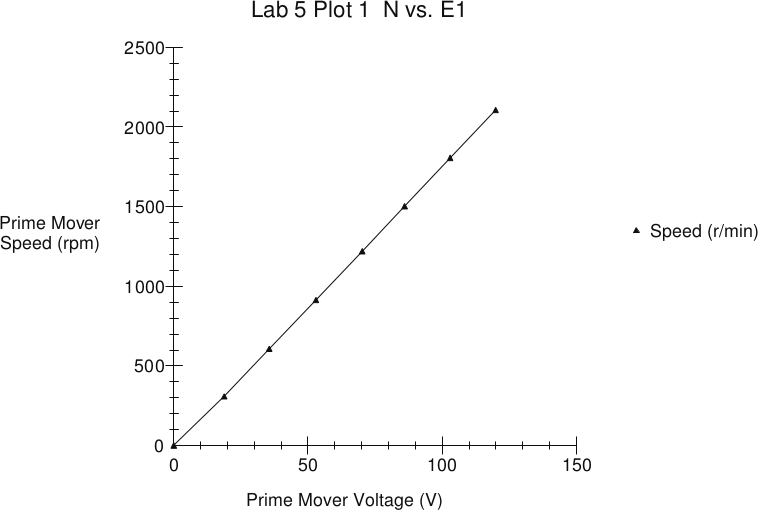
\includegraphics[width=\textwidth]{img/plot1}
  \caption{}
  \label{}
\end{figure}

\subsection{Dynamometer Operation}

\begin{table}[H]
  \centering
  \begin{tabular}{*{5}{c}}
    $n$ rpm & $T_{DYN}$ N-m& $T_{PM}$ N-m & $T_{NC}$ N-m & $T_C$ N-m \\
    \hline
    1500 &   0 & -0.66 &  --- &  --- \\
    1500 & 2.0 & -2.26 & 1.76 & 2.33 \\
  \end{tabular}
  \caption{}
  \label{}
\end{table}

\subsection{Motor Losses and Efficiency}
\begin{table}[H]
  \centering
  \begin{tabular}{*{7}{c}}
    \multicolumn{3}{c}{\textbf{Input}} & \multicolumn{3}{c}{\textbf{Output}}
    & \\

    \textbf{Voltage} & \textbf{Current} & \textbf{Electrical} &
    \textbf{Torque}  & \textbf{Speed}   & \textbf{Mechanical} &
    \textbf{Efficiency} \\

    &                  & \textbf{Power}      &
    &                  & \textbf{Power}
    & \\

    $E_1$ V          & $I_1$ I          & $PQS_1$ W           &
    $T$ N-m          & $N$ rpm          & $P_{m}$ W           &
    $A$ $\eta$ \\

    \hline

    88.71 & 0.94 &  89.90 & 0.32 & 1525.44 &  51.03 & 56.76 \\
    87.42 & 1.25 & 116.22 & 0.48 & 1474.08 &  74.44 & 64.05 \\
    86.08 & 1.58 & 144.32 & 0.67 & 1436.68 & 100.54 & 69.67 \\
    84.88 & 2.02 & 180.53 & 0.90 & 1394.14 & 131.70 & 72.96 \\
    83.98 & 2.40 & 210.73 & 1.11 & 1362.04 & 158.61 & 75.27 \\
    83.21 & 2.77 & 239.24 & 1.31 & 1340.72 & 183.39 & 76.65 \\
    82.42 & 3.13 & 267.18 & 1.50 & 1309.10 & 205.88 & 77.06 \\
    81.67 & 3.53 & 297.42 & 1.71 & 1273.63 & 227.89 & 76.62 \\
    81.01 & 3.90 & 325.22 & 1.92 & 1256.24 & 252.54 & 77.65 \\
    80.34 & 4.24 & 349.83 & 2.08 & 1232.10 & 268.29 & 76.69 \\
    79.57 & 4.64 & 379.02 & 2.30 & 1208.88 & 291.42 & 76.89 \\
  \end{tabular}
  \caption{}
  \label{}
\end{table}

\begin{figure}[H]
  \centering
  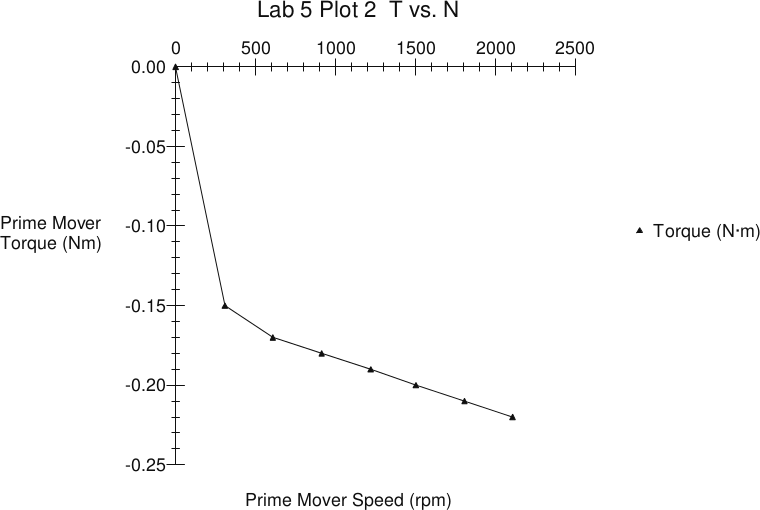
\includegraphics[width=\textwidth]{img/plot2}
  \caption{}
  \label{}
\end{figure}

\begin{figure}[H]
  \centering
  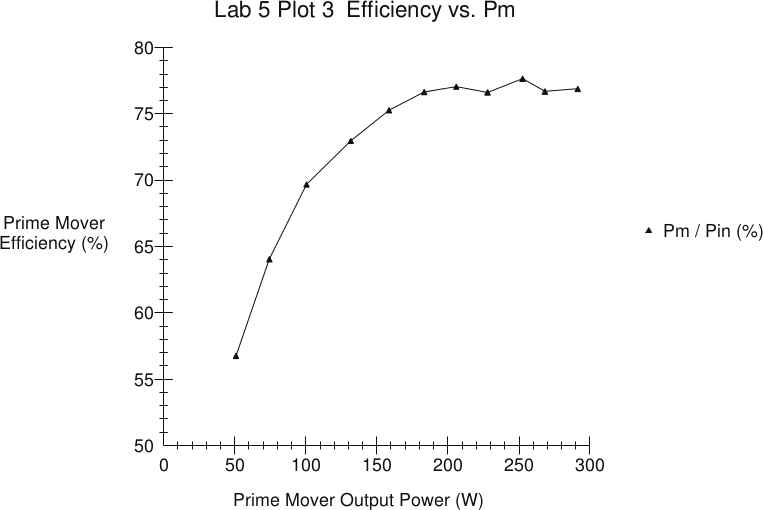
\includegraphics[width=\textwidth]{img/plot3}
  \caption{}
  \label{}
\end{figure}

\section{Conclusions}

% Note: The \label function lets you refer to whatever container it lives in
% with \ref.  You can see it's used every time we refer to a table or figure.
% You can also see that each \ref is preceded by a tilde, which is the symbol
% for a non-breaking space.
%
% So, if you want to refer to the section where Part 1 (\label{part1} was
% described, it'd look like: Section~\ref{part1} or \S~\ref{part1}
% \S is the symbol that means ``Section''.
The line and phase voltages of the source were measured in part 1. In
Figure~\ref{fig:circuit_01}, the three source voltages are in a
$\Delta$-connection, and hence the voltage values for each phase are the same
as the supply line-voltage.  When the voltages are added, they approximate 0-V
due to Kirchoff's voltage law. In Figure~\ref{fig:circuit_02}, the three source
voltages are in a Y-connection, and hence the voltage values for each phase are
$\frac{1}{\sqrt{3}}$ times the line voltage of 120-V.  When the voltages are
added, they approximate 0-V, since the connection is assumed to be balanced.
When the Phasor Analyzer was analyzed on the {PC}, it was confirmed that the
phasors were equal with 120 degrees phase shift for both the line and phase
voltage measurements. The fact that the addition of the phasors was not exactly
zero is most likely due to the fact that the voltage values measured were not
exactly equal to each other.

\section*{Equations}

\[P_{mech}\ =  (n \cdot T)\left(\frac{60}{2\pi}\right) \]

\section*{Circuits Tested}

\begin{figure}[H]
  \centering
  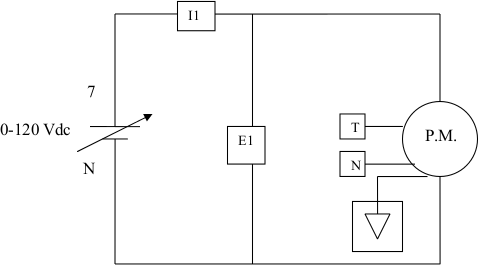
\includegraphics[width=0.8\textwidth]{img/circuit_01}
  \caption{Prime Mover Circuit}
  \label{fig:circuit_01}
\end{figure}

\begin{figure}[H]
  \centering
  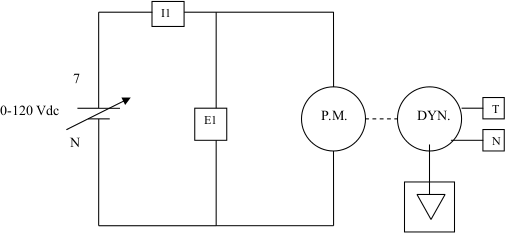
\includegraphics[width=0.8\textwidth]{img/circuit_02}
  \caption{Prime Mover Circuit}
  \label{fig:circuit_02}
\end{figure}

\end{document}
